% This is samplepaper.tex, a sample chapter demonstrating the
% LLNCS macro package for Springer Computer Science proceedings;
% Version 2.21 of 2022/01/12
%
\documentclass[runningheads]{llncs}
%
\usepackage[T1]{fontenc}
% T1 fonts will be used to generate the final print and online PDFs,
% so please use T1 fonts in your manuscript whenever possible.
% Other font encondings may result in incorrect characters.
%
\usepackage{graphicx}
% Used for displaying a sample figure. If possible, figure files should
% be included in EPS format.
%
% If you use the hyperref package, please uncomment the following two lines
% to display URLs in blue roman font according to Springer's eBook style:
%\usepackage{color}
%\renewcommand\UrlFont{\color{blue}\rmfamily}
%\urlstyle{rm}
%
\usepackage{listings}
\usepackage{xcolor}

\definecolor{codegreen}{rgb}{0,0.6,0}
\definecolor{codegray}{rgb}{0.5,0.5,0.5}
\definecolor{codepurple}{rgb}{0.58,0,0.82}
\definecolor{backcolour}{rgb}{0.95,0.95,0.92}

\lstdefinestyle{mystyle}{
	backgroundcolor=\color{backcolour},   
	commentstyle=\color{codegreen},
	keywordstyle=\color{magenta},
	numberstyle=\tiny\color{codegray},
	stringstyle=\color{codepurple},
	basicstyle=\ttfamily\footnotesize,
	breakatwhitespace=false,         
	breaklines=true,                 
	captionpos=b,                    
	keepspaces=true,                                   
	numbersep=5pt,                  
	showspaces=false,                
	showstringspaces=false,
	showtabs=false,                  
	tabsize=2
}

\lstset{style=mystyle}

\begin{document}
%
\title{Towards OGC API - Features centric GIS applications controlled by Object Relational Mapping}

%
\titlerunning{Towards an OGC API - Features centric GDI controlled by ORM}
% If the paper title is too long for the running head, you can set
% an abbreviated paper title here
%
\author{Olivier Monod\inst{1} \and Denis Rouzaud\inst{2}}
%
\authorrunning{O. Monod et D. Rouzaud}
% First names are abbreviated in the running head.
% If there are more than two authors, 'et al.' is used.
%
\institute{ Ville d'Yverdon-les-Bains, 1400 Yverdon-les-Bains, Switzerland \and
 OPENGIS.ch GmbH, 7031 Laax, Switzerland
}
%
\maketitle              % typeset the header of the contribution
%
\begin{abstract}
Most common GIS applications are composed of a spatially enabled database and a desktop client directly connected to it. In this configuration the business logic is often found either in the client application with custom plugins or in the database where many triggers are defined. When it comes to web GIS applications, a cartographic server is added in between the database and a web client. In this paper, we present an alternative setup where the data-model and the business logic are both defined in python programming language using the Django web framework ORM. Both desktop and web clients exchange data through OGC services.  In addition, the business logic is implemented in a middleware in a Django application. While mitigating the issues we face in standard PostGIS-based solutions, the Django ecosystem also comes with powerful tools offering interesting perspectives for such applications.

\keywords{ Geographic Information Systems \and OGC API - Features  \and Object Relational Mapping \and QField \and QGIS \and PostGIS \and Geo Data \and Infrastructure \and Django web framework.}
\end{abstract}
%
%
%
\section{Introduction}

GIS applications developers and integrators face the challenge of keeping a good operation to new feature development ratio. The operations cost can rapidly climb due to the ever increasing number of data synchronization and code maintenance tasks. Despite well documented, good infrastructure design and performant ETL softwares, it soon gets hard to keep operation overhead under control, lost in a sea of multiformat file based data exchanges and database models propagation procedures. In this paper, we detail one possible design that can help to keep operations costs under control. We illustrate the whole discussion with a real life example of gas and water network components in situ controls application on which we plan to apply this design in the future.

We compare the current architecture used with the future design that we imagine, based on tightly coupled Object Related Mapping (ORM) and OGC API - Features standards. In the end we acknowledge that GIS applications can take advantage of keeping as close as possible to web standards, creating specific tools only where absolutely necessary.

\section{GIS tools for utility management in Yverdon-les-Bains}

For a long time, periodic controls of the fluid network infrastructure have been done using paper forms that were then reported into a digital solution manually, inducing a significant and useless overhead. In order to digitize this work, looking for an Open Source solution, the QField option was high on the list of potential candidates. The usual setup would have been:
\begin{itemize}
	\item Setup an offline project, including local geodata.
	\item Send the field workers do the job with offline devices.
	\item Synchronize the new data back into the GDI using USB connection for data download and ETL script or sync plugin for data insertion into the database.
\end{itemize}



While this would have been easy to build for the GIS specialists, it wouldn’t have been as convenient as wished for the field workers due to the operations required back at the office to ensure new geodata ends at the right place. That is why the choice was made to use OGC Services as data sources for every layer on GSM connected devices, assuming full mobile network coverage over the working area. The resulting architecture removes all usual synchronization tasks.

It turns out that the solution worked well and that users adopted the new way of working quite easily. In 2023, a total of 4929 field controls of the water and gas valves were conducted by 4 technicians in charge of the pipe network infrastructure (fig.\ref{fig1}).

\begin{figure}
	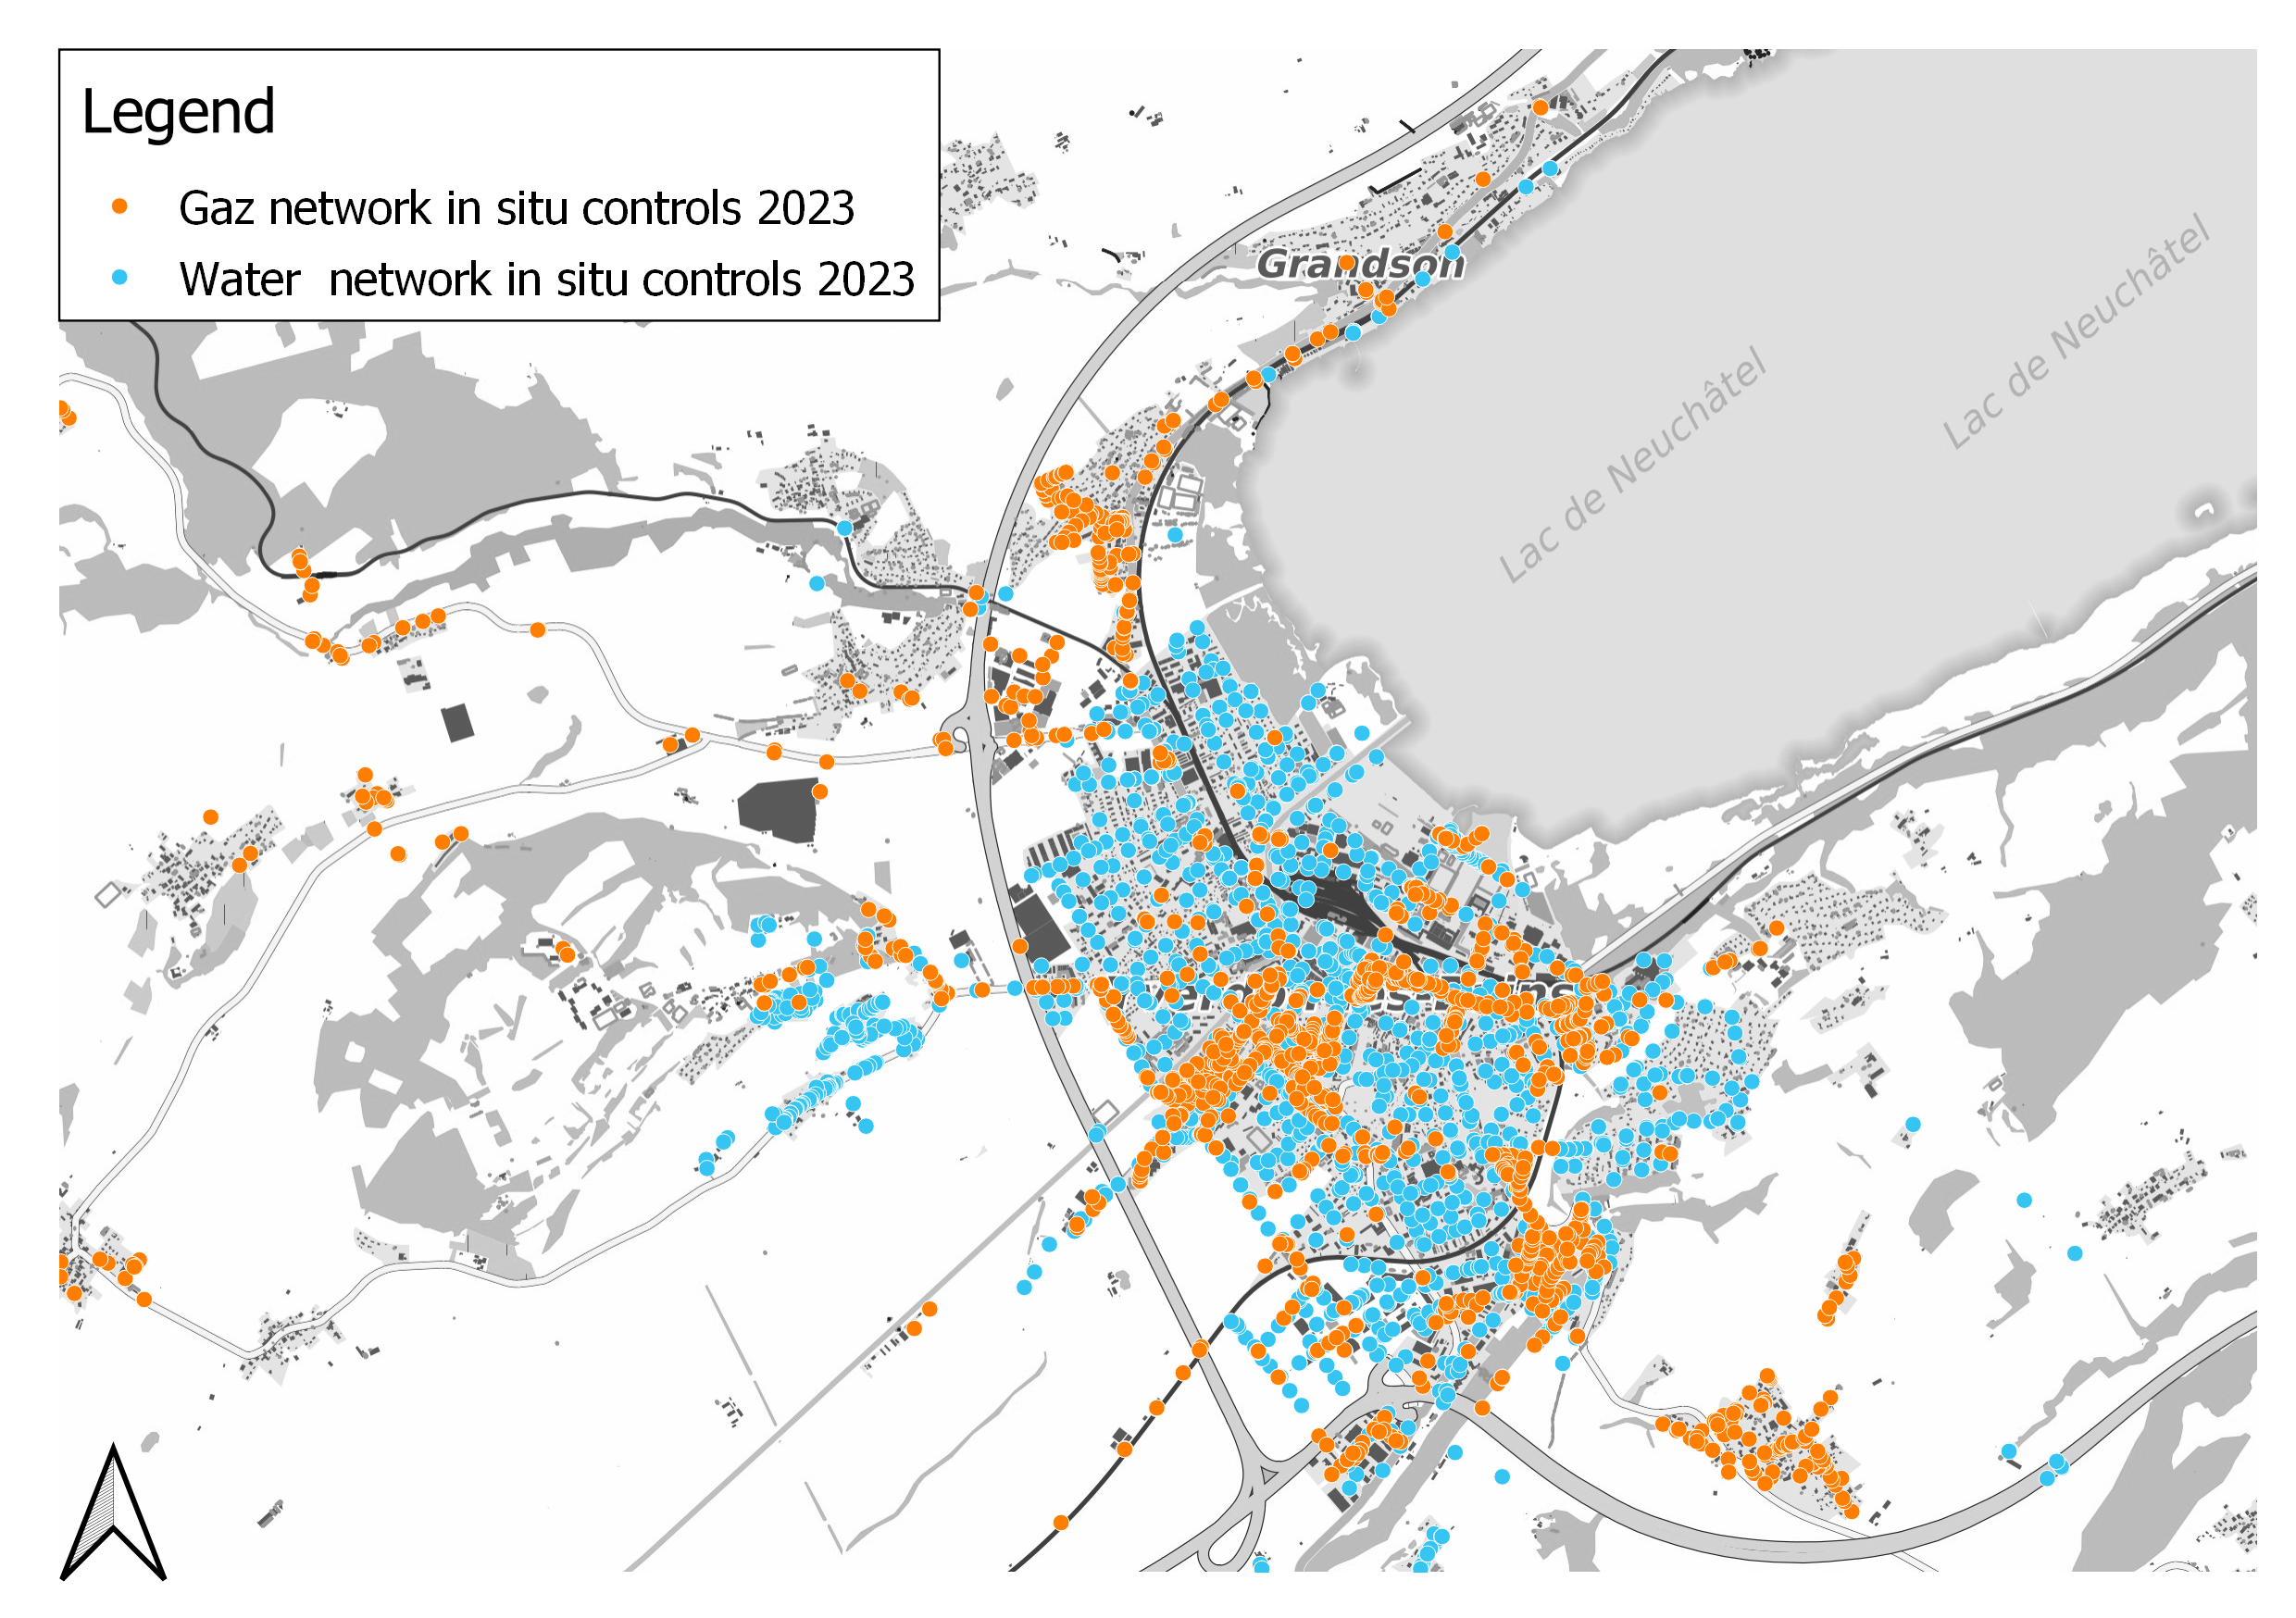
\includegraphics[width=\textwidth]{water_gas_2023.png}
	\caption{Map of in situ controls for gas and water network components in 2023} \label{fig1}
\end{figure}


\subsection{Results}

The good adoption of the solution and motivation of the field workers resulted in an impressive data collection over the three last years, reaching a total of 9344 field controls for the 2021-2023 years. This emphasizes also the excellent UX/UI proposed by Open Source mobile mapping solution QField\cite{ref_article3} (fig.\ref{fig2}).

\begin{figure}
	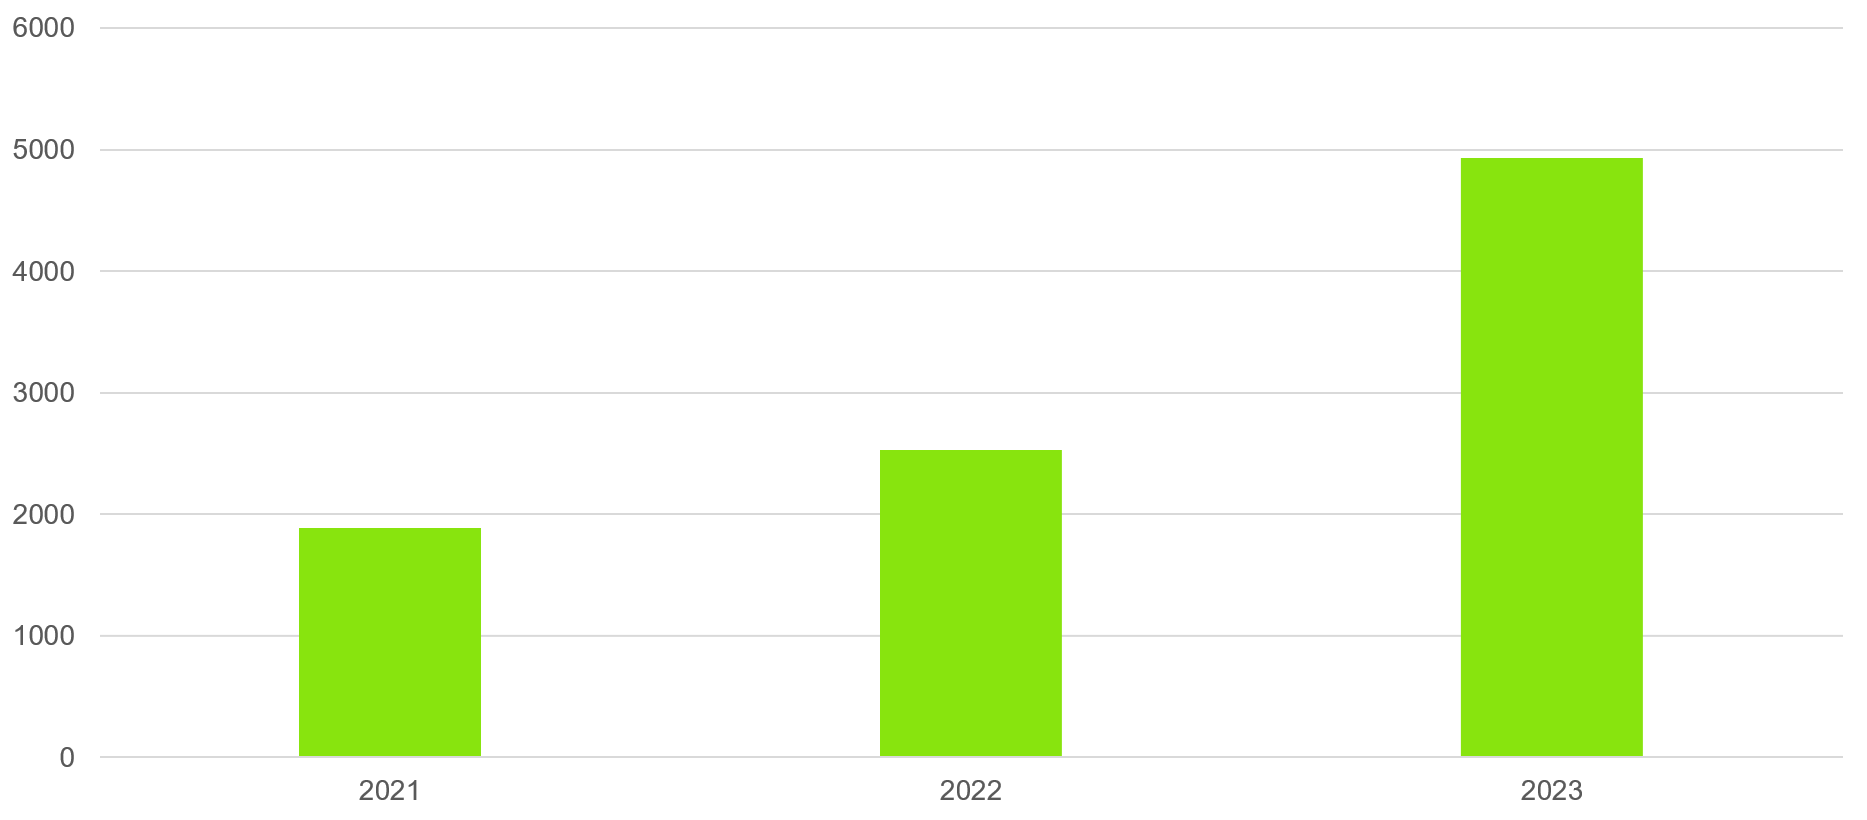
\includegraphics[width=\textwidth]{stats.png}
	\caption{Number of in situ controls per year} \label{fig2}
\end{figure}


\subsection{Current architecture}

\subsubsection{Description}

A quite usual architecture was designed at this time: OGC WFS 2 services is deployed using QGIS\cite{ref_article4} server connected to the postGIS database. Authentication and user management is done in Geomapfish Open Source geoportal\cite{ref_article1} in which a oauth2 backend have been implemented (fig.\ref{fig3}). The project was setup on the Geomapfish instance in Yverdon-les-Bains: Géoportail du Nord vaudois\cite{ref_article2}.

\begin{figure}
	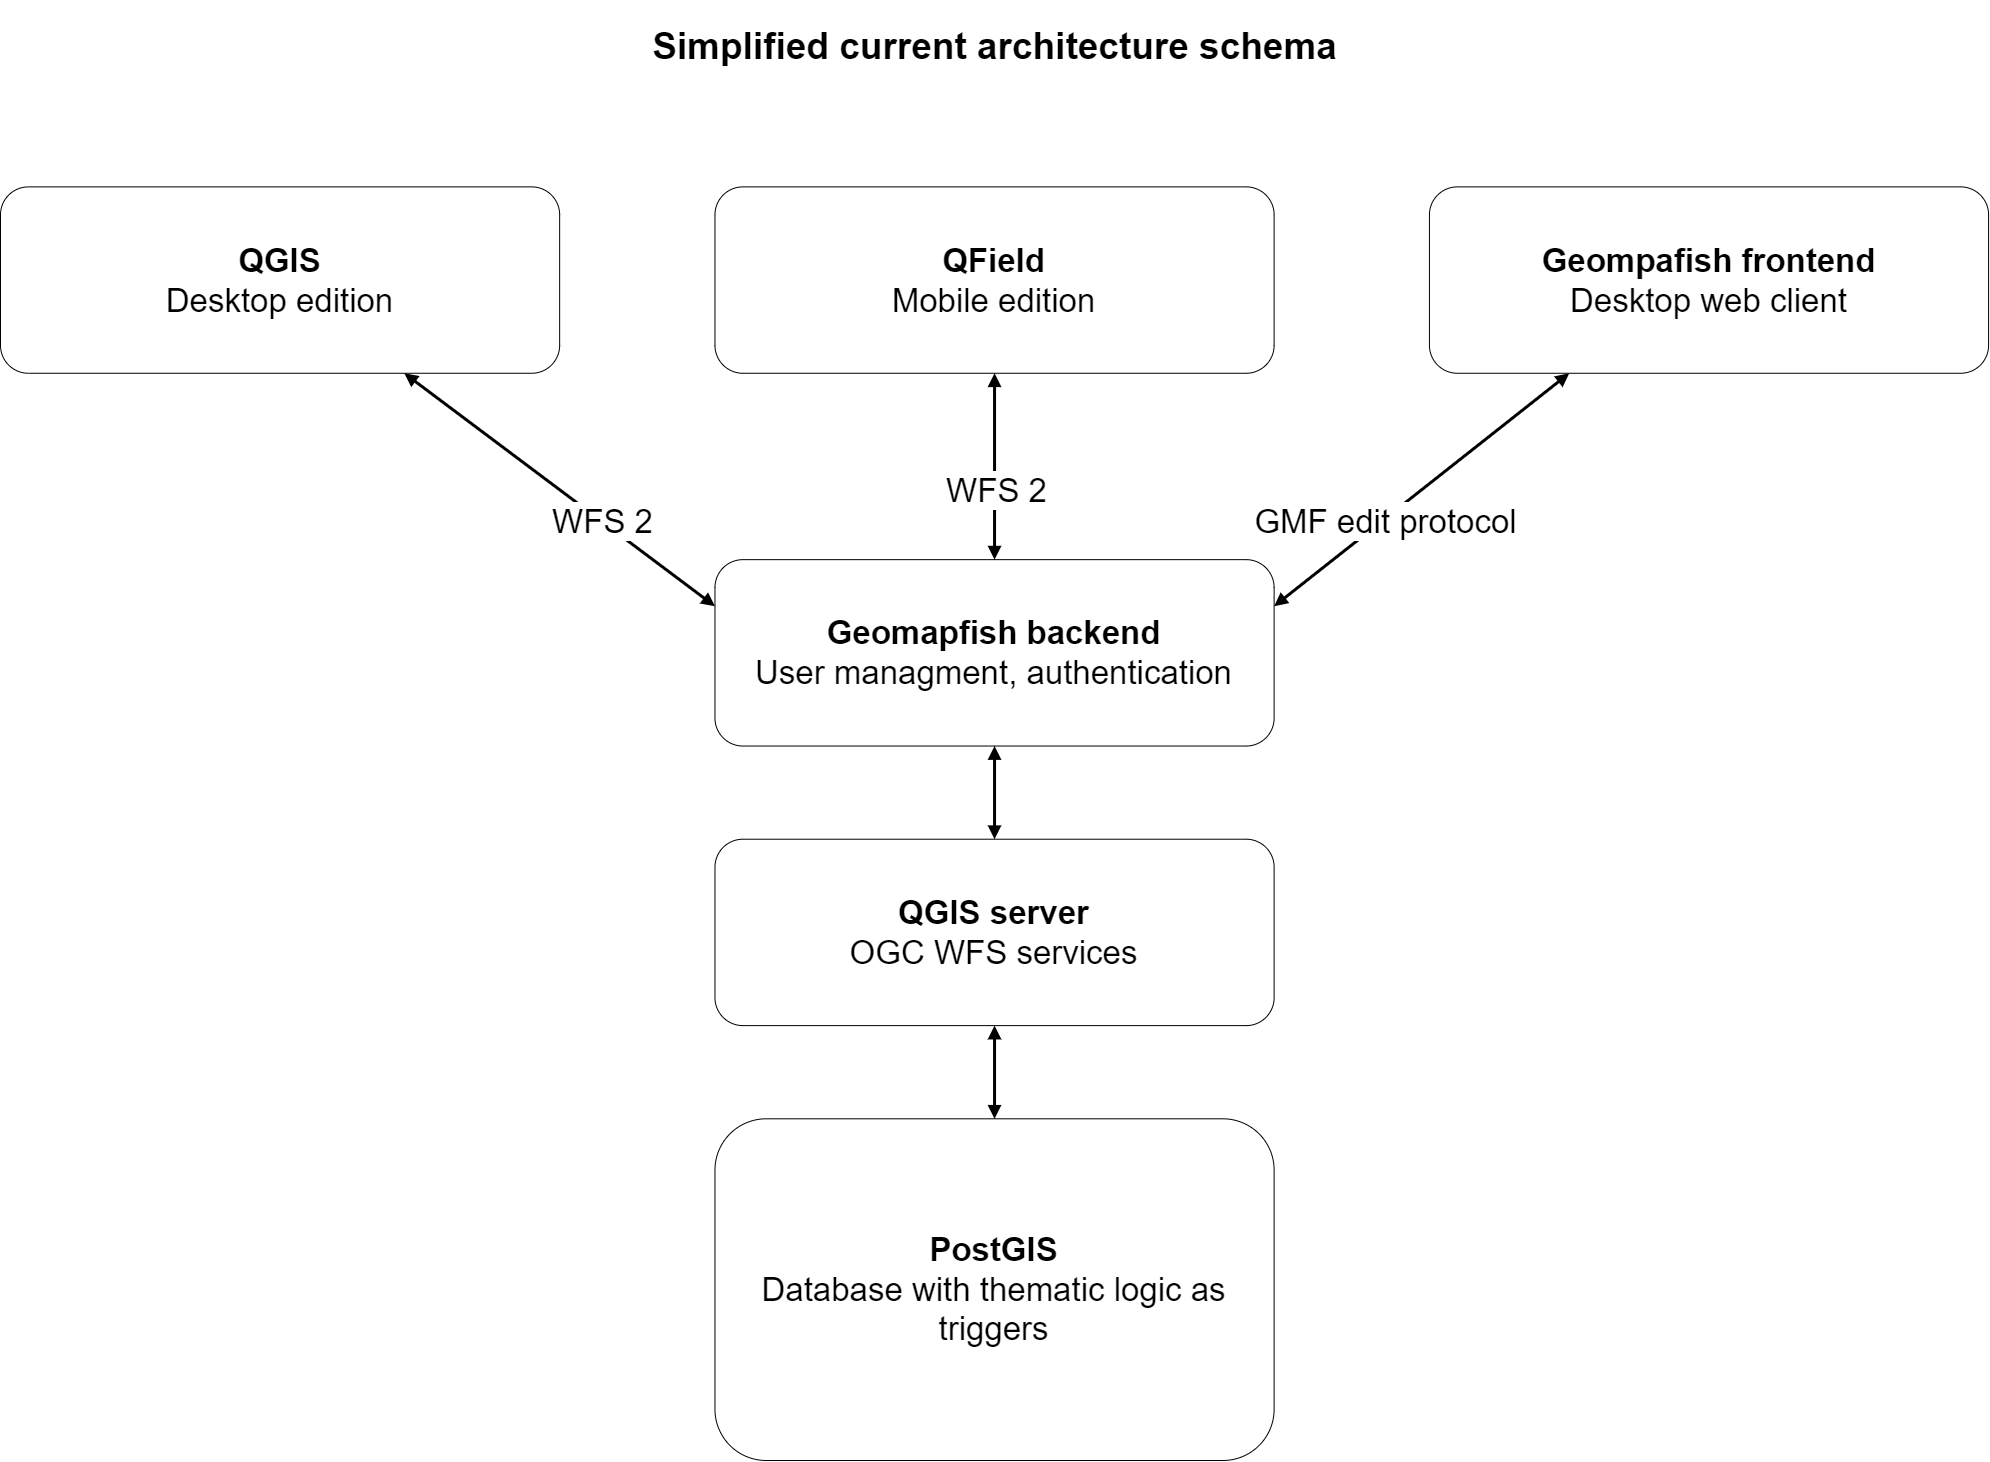
\includegraphics[width=\textwidth]{architecture.drawio.png}
	\caption{Simplified current architecture schema} \label{fig3}
\end{figure}


\subsubsection{Pros and Cons of the current architecture}

After a few years in production following advantages and drawbacks are identified.

\textbf{Pros} 
\begin{itemize}
	\item Low operations costs as almost no synchronizations tasks are required.
	\item Usual approach for development, no special programming skill needed. 
\end{itemize}

\textbf{Cons} 
\begin{itemize}
	\item No perfect debug tools, it's not easy to identified which layer of the stack causes problems.
	\item When adding new fields, value lists, etc... Many manual operations are required: edit database models, adapt the web services, adapt the qgis project, no unit tests.
	\item Even minor configuration (ex: adding a value to a list) task have to be done by the GDI administrators.
	\item The propagation of database models changes requires manual work for each instance. Manual adaptations of ETL scripts are also needed and no automation exists to notice the changes to dependent applications.
\end{itemize}


\section{The Object Relational Mapping Proposal with Django}

Django is one of the most popular web frameworks written in python that embrace the Don’t Repeat Yourself (DRY) programming principle: “Django makes it easier to build better web apps more quickly and with less code.”\cite{ref_article5}. The most important difference that distinguishes Django from other python frameworks is its integrated Object Relational Mapping which makes it particularly easy to work with complex data models and to manage models changes (migrations) efficiently. Furthermore as for the whole framework, the ORM documentation is of very high quality. Besides, Django ships with lots of features that can be useful in any GIS application: 

\begin{itemize}
	\item Integrated security.
	\item Out-of-the-box administration interface with user management. 
	\item Authentication.
	\item Popular and well maintained packages such as: multi-tenant; simple historization; oauth clients, oauth backend.
	\item And last but not least to us: GIS enabled data model with GDAL/GEOS integration.
	\item Spatial extension of Django Rest Framework
\end{itemize}


\subsection{Controlling a Geo Data Infrastructure with an Object Relational Mapping: what’s the benefit ?}

 Django ORM and migration tools offer a structured, controlled way to manage the database models and maps these models with corresponding python classes. Thus, the models definition is done in python using Django syntax. Any model change will then have to be made on the python class and will be then materialized in the database using the migration tool. Introducing middleware between the webservice and the database allows the developers to implement business logic without the need of adding triggers in the database or developing specific plugins in the client. As an example, for electric network GIS, the application has to ensure that when a tube linestring is divided, related cables linestrings also get divided in a coherent manner.

Many Open Source solutions support OGC API - Features service deployment, among them: QGIS server; mapserver; geoserver; and for python enthusiasts: pygeoapi. At this point, one could question the rational for a new development. 

Without this new tool we would miss some interesting features: easy way to work with complex database relations; easy resolution of value list; avoid writing raw SQL that is difficult to maintain.

But the most important aspect with the perspective of building complex GIS applications is that if we connect one cartographic server directly to the Postgis backend, we are losing the entire business logic offered by our middleware approach, making it a bad solution for applications that do more than publishing layers or editing basic data models.
 

\subsection{The django-oapif package: single liner OGC service deployment}

With the objective of replacing complex network management solutions in the future, a Proof of Concept\cite{ref_article6}\cite{ref_article7} has been realized by OPENGIS Gmbh in 2023. The goal was to validate the direct deployment of a Django model as an OGC service and identify potential limitations.

\subsubsection{Development}

The result is very efficient in terms of coding simplicity. The new Django package allows to deploy an OGC API - Features service with a single line of code placed on top of the model definition as in the following example. With such a tool, it is quite easy to build a new infrastructure (fig.\ref{fig4}).

\begin{lstlisting}[language=Python, caption=Python code sample]

from django.contrib.gis.db import models
from django_oapif.decorators import register_oapif_viewset

@register_oapif_viewset(crs=2056)
class SwissMunicipalities(models.Model):
id = models.UUIDField(
	primary_key=True,
	default=uuid.uuid4, 
	editable=False)
name = models.CharField()
geom = models.MultiPolygonField(srid=2056)
\end{lstlisting}


\begin{figure}
	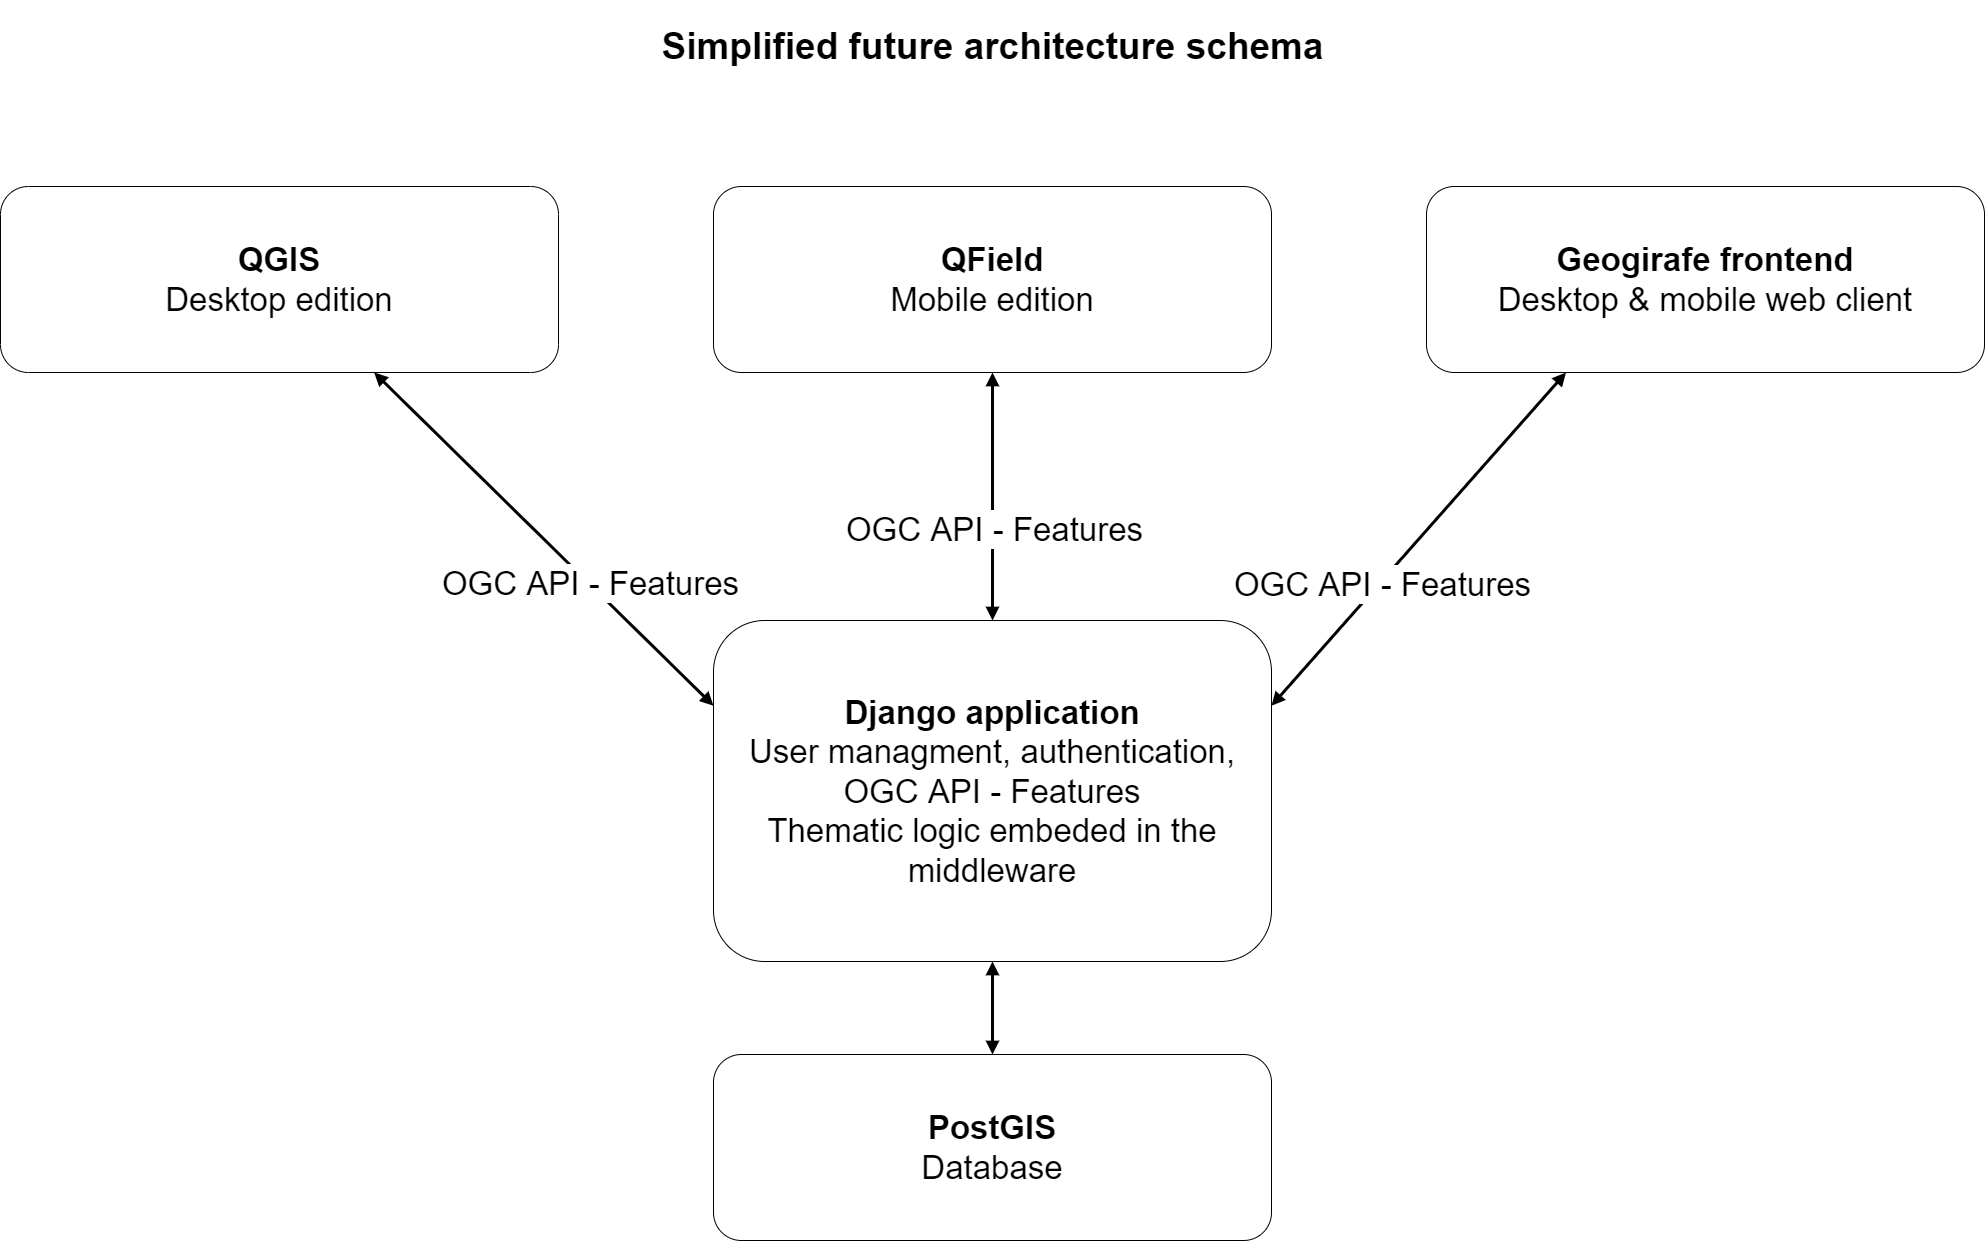
\includegraphics[width=\textwidth]{future-architecture.png}
	\caption{Simplified future architecture schema} \label{fig4}
\end{figure}


\subsubsection{Performance}

Since the start of this project, we have been expecting some poor performance in terms of reading time. Fetching a complete layer (known as a collection in Django) might take quite some time (fig.\ref{fig5}).

\begin{figure}
	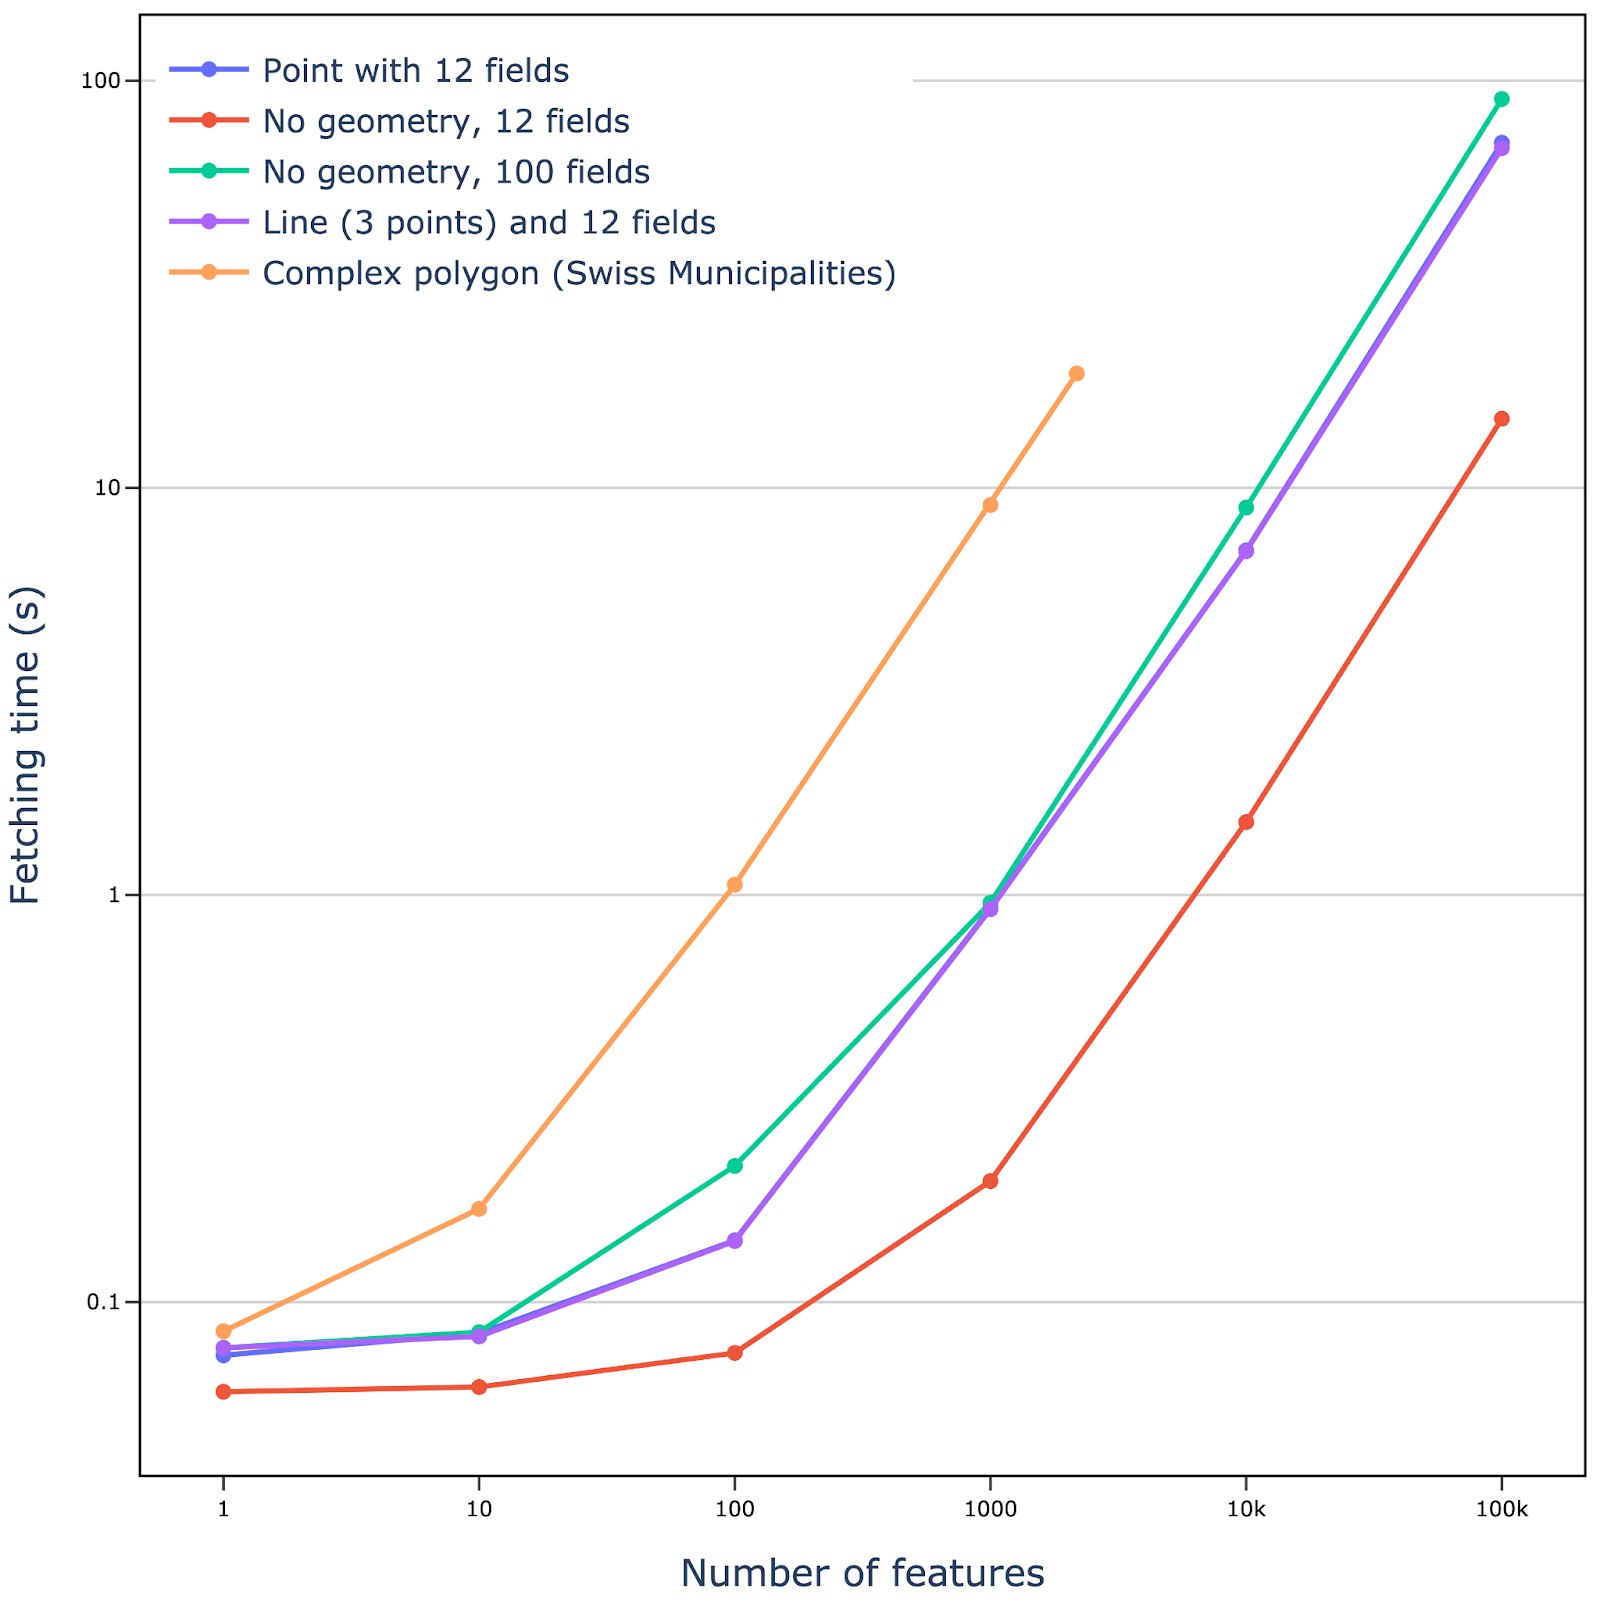
\includegraphics[width=\textwidth]{benchmarcka.png}
	\caption{Benchmark of feature fetching time} \label{fig5}
\end{figure}

As we could have expected, the fetching time is becoming linear after a certain threshold, between 10 to 1000 features depending on the complexity of the serialization.

Profiling showed the serialization of the geometry was a significant part of the cost. Here serialization consists in turning the binary geometry representation into, roughly, a JSON list of coordinates. Instead of achieving this in Django, we tried to delegate this process to Postgis by using one of its native function. This gave very satisfying results (fig.\ref{fig6}).

\begin{figure}
	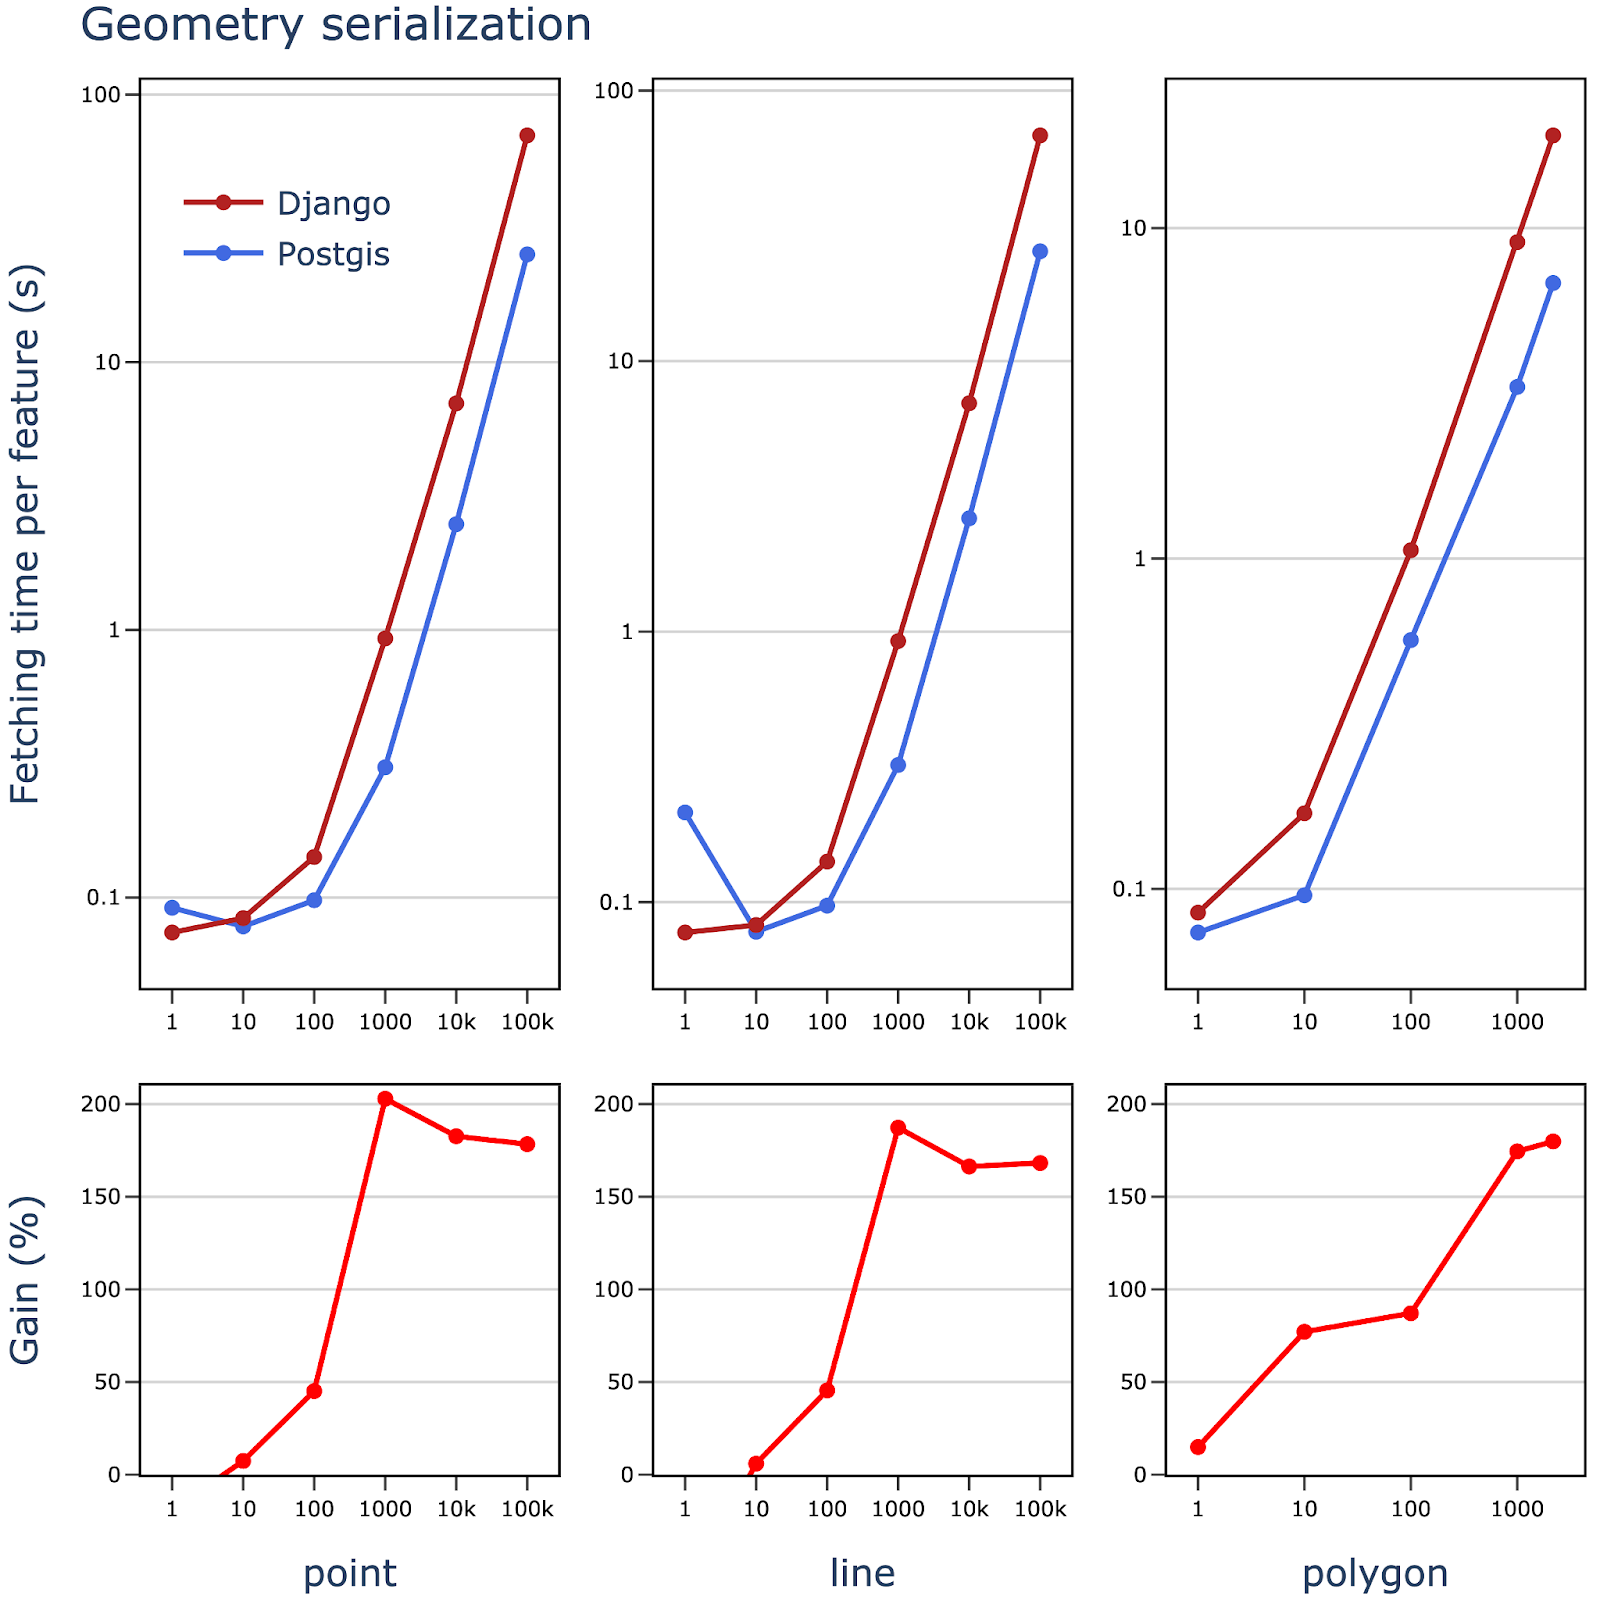
\includegraphics[width=\textwidth]{benchmarckb.png}
	\caption{Benchmark of geometry serialization} \label{fig6}
\end{figure}

Depending on the number and type of features, the gain is within 50 to 200\%.


\section{Conclusion}

Using an ORM and django-oapif will require a little more coding literacy from GIS application integrators than before. But in return, maintenance costs of business logic that is distributed in plugins or in the database will sink. Futhermore, GDI administrators will gain better control over the data structures and their evolution making it more robust and understandable. Introducing this middleware approach in GIS applications enable the centralized implementation of complex business logic in a  well defined manner and simplifies update process. With the emergence of this architecture design, we hope the gap between advanced desktop GIS solution and web GIS or mobile applications will reduce.



\begin{credits}
\subsubsection{\ackname} Django-oapif Proof Of Concept development was funded by: Ville d'Yverdon-les-Bains, Ville de Morges, Ville de Nyon

\end{credits}
%
% ---- Bibliography ----
%
% BibTeX users should specify bibliography style 'splncs04'.
% References will then be sorted and formatted in the correct style.
%
% \bibliographystyle{splncs04}
% \bibliography{mybibliography}
%
\begin{thebibliography}{8}
\bibitem{ref_article1}
Geomapfish: https://geomapfish.org
\bibitem{ref_article2}
Géoportail du Nord vaudois: https://mapnv.ch
\bibitem{ref_article3}
QField: https://qfield.org
\bibitem{ref_article4}
QGIS: https://ggis.org 
\bibitem{ref_article5}
The Django web  framework: https://www.djangoproject.com/ 
\bibitem{ref_article6}
Django OGC API - Features by Opengis: https://github.com/opengisch/django-ogcapif
\bibitem{ref_article7}
Django DRF GIS: https://github.com/openwisp/django-rest-framework-gis
\bibitem{ref_article8}
Geodjango: https://docs.djangoproject.com/en/5.0/ref/contrib/gis/



\end{thebibliography}
\end{document}
